Considering the state of the art, there are several approaches that face the 
problem described in previous section. The key point is to find a simple and 
effective way to extract API functions call and build a recommendation system 
able to provide developers with very suitable recommendations with respect to 
the developer context. Even though several techniques and tools have been 
proposed over the last decade, most of them share the main activities shown in 
Fig. \ref{fig:apiRecommendationExistingApproaches}. In particular, the 
developer context consisting on source code files is analysed to obtain 
corresponding ASTs. The retrieved abstract syntax trees are taken as input by a 
similarity analysis step in order to retrieve from the available knowledge the 
cluster of API client source codes that share some similarity with the code the 
developer is working on. Subsequently, a ranking activity is performed in order 
to finally recommend the developer with source code fragments that on one hand 
are similar to the developer context and on the other hand permits to grasp how 
other existing projects use the considered APIs. In the following, 
representative approaches implementing the process shown in Fig. 
\ref{fig:apiRecommendationExistingApproaches} are presented and compared at the 
end with respect to a set of specific characteristics.




%So far, we have seen several approaches to perform recommendations related to 
%API context. The proposed tool from the literature are very different from the 
%point of view of dataset, similarity measure and clustering techniques but 
%they 
%share a conceptual model that starts from the abstract syntax tree of the code 
%to the final recommendations. This procedure is depicted in Figure 1, that 
%describe at high level the main steps to reach the final output. Many of these 
%are optionally but, as we have seen in the previous discussion, are strongly 
%recommended to perform a better analysis and to have good enough results.
%For the proposed approach, we choose to combine the results coming from CLAMS 
%with the code cloning technique, by using Simian. Basically, we propose 
%something that is different from the existing approach analyzed. For example, 
%we avoid to use clustering techniques because we rely completely on Simian for 
%this task.  

\begin{figure}[!h]
	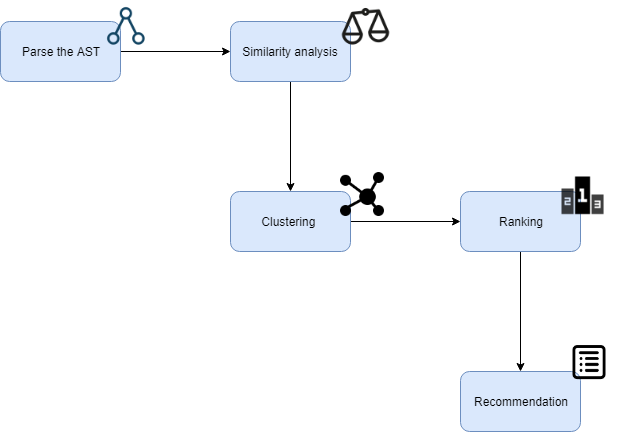
\includegraphics[width=12cm,height=14cm,keepaspectratio]{images/approach.png}
	\centering
	\caption{Main activities shared by existing techniques to provide 
	developers with API recommendations}
	\label{fig:apiRecommendationExistingApproaches}
\end{figure}






%To this end, several approaches are available able to 
%analyze the developer source, to adopt some similarity metrics, and to 
%optionally apply clustering techniques for representing the obtained results 
%in 
%the form of recommendations that should be clear and effective. 

%approaches that follow the same main skeleton to solve the problem; what is 
%different among them are the techniques, algorithms and produced results but 
%they are all useful and give the flavour of the API call function problem. 



\section{API mining framework: MAPO}
In~\cite{zhong_mapo:_2009} the authors propose MAPO that perform methods extraction using data mining techniques, clustering them to have a more representative data and build a recommender through GEF tool. So, they divided the process into three main steps: analyzing the source code, the API miner and API recommender. First of all, MAPO parses the source code coming from Java Github projects that use Eclipse Graphical Editor Framework (GEF), using JDT parser utilities that allow to analyze in deep a Java file and extract classes, interfaces, method invocations and method declarations. For the recommendations, MAPO considers as API method suitable for the recommender only those belong to third-parts libraries, considering the GEF framework as external, class cast and creation associated to external class and the method call that belongs to external class; basically, the authors ignore the libraries and so the internal API of the JDK. Then MAPO collects all source code by using @ as initial mark to identify a method call and \# as separator between method and related class. \\
This format is called ARFF and we will explain it in the related section. About the conditional statements, such as if, while and so on, the authors not considered the possible relations among multiple conditions and in practice the represent them as flat code in which MAPO considers all branches. As claim by authors, this simplification is necessary otherwise the mining phase is infeasible and the API recommender is not effected by them. Once the method calls are selected, there is the problem of method overweight and common-path overweight that involves respectively several method calls and sequence in common in the source code that can introduce bias in the result; for example, in fragment of code MAPO can select a method call only because it is replicated and not for its real effectiveness. To avoid this problem, the authors select the longest sequence in common that covers also the smaller sequence of method call and, in this way, the reduce the bias. Moreover, MAPO selects only third-parties libraries using inline methodology, that consist to explore the parse tree of classes and identify the ancestor and so excluding the JDK methods. \newline
Once MAPO have all method call, the next step is mining the sequence to produce recommendation. To do this, is not enough to consider all method sequences because this can bring incorrect results. So, MAPO using first similarity metric, based on the name and the usage of methods to identify similar sequence and then clustered them by using data-driven hierarchical clustering. In particular, the authors consider three level of similarity given by class names, method names and called API method and obtain in this way the similar sequence. Then, by using Mathlab tool, MAPO performs classical hierarchical clustering to obtain the ranked list of representative sequences, transform them into transaction and put them into a database. Finally, the API recommender is a Eclipse plugin that allow developer to click on the method of interest, execute a query on DB to show possible uses by using sample code and developer can also see details on the proper window tab in which the API method are highlight.\\
 To validate this approach, the authors use a dataset composed by 20 projects that used Eclipse GEF, run the tool and show the effectiveness of their approach by a quantitively comparison. To reinforce the validity, they also conduct an empirical study on by considering a set of tasks to do and select a group of Java developers that is involved to solve those tasks.


\section{Mining succinct API usage patterns: UP-Miner}
A similar approach is performed by~\cite{wang_mining_2013} in which the authors create UP-Miner tool that improve MAPO in term of accuracy. Going in deep, the aim of the authors is to achieve the succinctness but also the effectiveness of mined pattern that represent an enhancement of previous approach. Once the authors define API usage mining, that is the optimal number of patterns under a given threshold, they propose a clustering technique based on BIDE algorithm. As first step, UP-Miner extracts API pattern sequences using Roslyn AST parser from the projects that compose the dataset. Then, the apply the SeqSim n-gram technique that takes two sequence computes the similarity that is based on the shared items between them in term of objects and classes used and on the longer and consecutive sub-sequences rather than the shorter ones. This phase produces weighted results that are used for clustering that are conservative on, in sense that the maximum distance between two cluster is the maximum distance between two elements of those cluster.\newline
Then, UP-Miner use BIDE algorithm, that have the key concept of frequent sequence: a general sequence became frequent if its super-sequences (namely the sequences that contains the considered sequence) is greater or less of the given threshold. Consider this, BIDE algorithm can extract the longest common sequence that are useful to divided the results into different clusters, but it is not sufficient because at this point there may be some redundant cluster. So, it is necessary to apply once again the previous phase considering the cluster as usage pattern and this two-step clustering grants an improvement in term of redundancy considering also two different threshold (one for pre-BIDE and another for post-BIDE application). Until this, UP-Miner address the problem of coverage but the aim of the authors is to reach also the succinctness of patterns. To do this, UP-Miner use a dissimilarity metric that measure the diversity of a usage pattern from another and an utility functions to maximize in order to obtain the better results, decreasing the threshold at each step of the algorithm implemented for this task. \\
Once UP-Miner computes the correct and more succinctness as possible usage API pattern, the authors show them to the developer by building a probabilistic graph in which each node is a usage pattern and the edge is weighted with certain probability. To produce this prototype and make some experiments that involves the developers in a similar way as we see in MAPO, the authors use a very large C\# dataset as input files and compare their results with MAPO ones.

 


\section{Summarizing API with clustering techniques: CLAMS}
Go further with the examination of the existing approaches, we have also CLAMS tool proposed in~\cite{katirtzis_summarizing_2018} that follows a quite similar approach but it differs from the point of view of the results. In fact, CLAMS produces as API recommendations snippet of code that represents a pattern for a certain library. As usual, the preprocessing phase is done by analyze the AST of the source code (in case of CLAMS, projects related to 5 popular Java libraries) with a depth-first search using JDT as previous example. This phase produces snippet of code that brings all information about API implemented in the code. The similarity technique is based on Longest Common Subsequence (LCS) and is more effective rather than an analysis at source code level. By using this technique, CLAMS creates a distance matrix that is used as input by the clustering module of CLAMS, that implements the hierarchical version of DBSCAN algorithm, called HDBSCAN, plus a post-clustering processing to eliminate the sequences that are identical to snippets for each cluster obtained. The aim of HDBSCAN is to isolate the less representative methods and, more in general, points into a distribution that are really far from the rest of the dataset. \\
To do this, the algorithm uses a distance called core distance to draw a circle on the points to exclude and then computes the mutual reachability distance that reduce the presence of sparse node in the dataset. Then, by applying Prim's algorithm, HDBSCAN calculates the minimum spanning tree among the closer nodes and finally sorts them by a hierarchical clustering (this phase is not present on the original DBSCAN algorithm), as well explained in the related work. There is also a useful Python library used in CLAMS that provides utility functions to make all this step in a very understandable way. The core module of CLAMS is represented by the snippet generator, that performs six main steps in order to obtain the final snippets that represent patterns. First of all, CLAMS replaces all literals present in the code with their abstract type by using srcML, a tool that produce XML file starting from a source code, and removes all comments. At the end of this step, we have code with the same structure of the original source file but more abstract.\\
 Then, CLAMS identifies API call in that code and what are not related to them and creates two lists. In the next step, the authors identify all variable in the scope of the API sequence. To finish the process, the non-API statements are removed and they put on top of snippet variable declaration related to API, plus of course the snippet of code related to those API. So, the snippet of code that is produced in this way is composed by a sequence of variables related to API class and a possible use of them, with considering also the statements present in the original code (CLAMS retained also the structure of the code). The authors put a comment Do Something in the section of code in which the founded variables may be used. \newline
Once CLAMS has these results, the snippet selector module finds for each cluster the most representative snippets by giving them a score. To do this, 
the authors use another algorithm that works on AST, called AP-TED that creates a distance matrix between two clusters and from this, calculate the similarity. Finally, CLAMS ranks all representative snippet using the definition of snippet support define as follow: a snippet is supported if there is a file that contains a supersequence of it. An example of extracted pattern is depicted below and it is related to Twitter4j, a library that allows connection with a twitter client. 
\begin{lstlisting}
{
    AccessToken accessToken;
    final String CALLBACKURL;
    RequestToken requestToken;
    SharedPreferences prefs;
    Twitter twitter;
    twitter = new TwitterFactory().getInstance();
    twitter.setOAuthConsumer(OAuthConsumer.CONSUMER_KEY, OAuthConsumer.CONSUMER_SECRET);

    if(!prefs.contains(string) | !prefs.contains(string)) {
        try {
            requestToken = twitter.getOAuthRequestToken(CALLBACKURL);
            String authUrl = requestToken.getAuthorizationURL();
            // Do something with authUrl
        } catch (TwitterException e) {
            Toast.makeText(this, e.getMessage(), Toast.LENGTH_LONG).show();
            Log.e(string, e.getMessage());
        }
    } else{
        accessToken = new AccessToken(prefs.getString(string, string), prefs.getString(string, string));
        twitter.setOAuthAccessToken(accessToken);
    }
}
	
\end{lstlisting}

Moreover, for human readability reason, CLAMS beautifies snippet using A-style tool, that removes useless spacing and fixes the indentation of the final snippets. For the evaluation task, the authors use 5 popular Java libraries coming from Github projects and they are Apache Camel, Drools, Restlet framework, Twitter4j, Project Wonder and Apache Wicket. In the evaluation section of their paper, the authors taking into account different clustering algorithm and make experiments with HDBSCAN, already mentioned, k-medoids that is similar to the previous one but achieve more coverage but less precision. This algorithm is based on find a central point that has the equal distance from the rest of the point, called medoid. \\
In our case, the medoid is a particular method API call that is the most representative for the library. K-medoid algorithm uses also n-gram based technique and similarity distance matrix as HDBSCAN. To answer to the research question, the authors of CLAMS preform also a comparison with NaiveSum and NaiveNoSum approaches, that are clustering techniques less precise with respect to the HDBSCAN and K-medoids. In fact, the better results are coming out from the latter algorithms. \\
Furthermore, the evaluation is composed by a user survey about the utility and real support given by CLAMS patterns. All this information are available at the CLAMS official site, that contains also the Github project, the original dataset and the instruction to set up the environment to launch CLAMS as standalone platform on Linux machine. As claimed by authors, this work is really interesting and flexible because it is not dependent on a specific program language. The only constrain regarding the srcML tool to produce the XML files related to API patterns, but it is not a big issue from the adaptation point of view, as we can see later.



\section{API recommendation with statistical learning: APIrec}

APIrec tool~\cite{nguyen_api_2016}, instead, uses statistical techniques in order to keep trace of the context in which a developer writes its own code, by analyzing the co-occurrences and fine-grained code changes. Differently from the previous approaches, the authors keep trace of the context in which the API method call may be useful. As usual, to extract the source code from the 50 Java projects randomly selected from Github, APIrec navigates the AST of the source code using GumTree tool. Before going in deep with the implementation, the authors give several definitions that are useful to understand the behaviour and the contributions to the state of the art given by APIrec. \\
First of all, the term API for the authors indicates both external and internal method calls and APIrec performs recommendations only if the context of API is correct for a certain situation. Regarding the AST, we have the atomic change that represent a new element on AST composed by kind of operation, AST node and label. A collection of atomic changes is called transaction and is stored in a bag, a particular data structure that we commonly find in the AST definitions. An important concept that is a key definition for the APIrec implementation is the code context, represented by code tokens related to the API that the developer is writing. Taking into account the tokens, the authors consider both the distance and the order of this, as an API method calls have a specific call order and they are really effectiveness only if there are called in the proper way. To remark this feature, APIrec gives also a weight based on how near the token by is considering the distance matrix. Once they define this set of metric and concept, the authors show the inference model based on likehood scores taking into account both change of the context and code.\newline
The entire model is based on the correlation between a code token and another, expressed as we said in term of atomic changes in the AST and transactions. In particular, APIrec evaluates the probability that certain events, namely the transactions, occurs given another. This score is called association score and it is used to calculate the distance between two changes into the code as well as new methods that will take a part in the final recommendation. \\
At the end of these computations, all possible scores and weights are calculated but it is not enough to perform the recommendations. In fact, it is necessary to apply machine learning techniques in order to train APIrec with the code changes and context. To do this, the authors use hill-climbing adaptive learning filled with three parameters: numbers of co-occurrence founded with fine-grained atomic changes, numbers of co-occurrences related to changes tokens and two weights. With this process, the necessary scores are calculated and APIrec is able to perform the recommendation by considering the most probable method calls for a certain API. The methods are also ranked by highest probability of usage but also distance, scope and dependency are considered in the ranking phase. To support their tool, the authors conducts several experiments over a very large dataset, including also analysis regarding code change context, user empirical studies, evaluation of accuracy and predictions.



\section{Synthesizing API usage examples: Buse-Weimer algorithm}
Paper from Buse and Weimer~\cite{buse_synthesizing_2012} is still about API call but is focused to produce automatically a documentation for the projects in a human readable format.
Once they obtain data from mining phase, the proposed algorithm extract API pattern and rearrange them in a more readable and effectiveness format. The focus of this work is on Java documentation that provides useful hints and suggestions when a developer is implementing an API functionality. Although in general the Java doc helps in this kind of activity, it often lacks in something, as the examples are too general or it not able to give a concrete hint for the problem that the developer is trying to solve. So, the aim of the authors is to produce an enhanced version of documentation that is really useful for the developers, starting from retrieve the API patterns, defined as the sequence of function call for a certain API class, called target class. \\
Once this first step is done, the algorithm tries to produce a human-written documentation for the API, taking into account some characteristics such as the lines of code, that are 11 on average but 5 for the median. Moreover, the authors consider also the abstract initialization, abstract usage and exception handling. All this information is extracted using JDK utilities and they are validated by the authors, putting more effort on the human aspect. To validate the results, they involve over 150 developer and collect their answers about the proposed results. By analyzing these statistics, a typical developer wants multiple uses for a certain class or API method and not only one, that may be not useful for his particular context. Another key point is the conciseness of the suggested snippet of code, as well as the readability and variables names that must be related to the context, also including temporary ones to improve the readability. So, from this survey, we can identify four key points to achieve the human-written documentation: size of the code, readability, representativeness and concreteness.\newline
To reach these goals, we can look to the algorithm implementation, that the authors divide into four main step: the path enumeration, predicate generation, clustering and finally the output documentation. Starting from the path identification, they scan the code and identify acyclic part of the code that represent a path for the target class. Notice that this approach can led some bias but it happens in practice and the authors choose to stay close with respect to real implementation. \\
So, they use intensively human users to perform test and to measure the accuracy of their proposed algorithm. As the previous approaches, they parse the code and cluster the significant result with a distance matrix in order to build the related documentation. As the purpose is different from previous works, they are adding some clustering also on predicate and represent the abstract pattern as a graph. Then they compute symbolic execution over these paths on order to produce inter-procedural path predicates that are logical formulas used to represent the code and in particular, if a certain statement is reachable or not. From this abstraction, the algorithm computes use seeds that are local instantiations of fields, objects and whatever is related to the target class. Finally, from these it produces concrete uses, the real hints about the target class, that are stored in graph form in which edges keep trace about what happens before and so, in this way, we have the context as well as the chain of methods necessary to implements the features related to the target class. \\
To have better results, however, it is not enough to produce usage examples, as we seen so far with the other related works. Clustering is necessary to avoid heavy computation, and the proposed algorithm exploits the well-known k-medoids algorithm with some modifications, as the original algorithm is not suitable to detect distance about objects. The distance matrix that is taking into account by the k-medoids algorithm is based on the happens before relation obtained from the graph. So, at the end of this computation, the algorithm obtains the cluster and summarize them into abstract uses, represented once again in graph form. \\
The final step of the proposed algorithm is to produce the documentation. Starting from the abstract uses, it uses a topological approach to avoid the cycle and branches that appear in the code, as the final recommended documentation about the target class must be a flat file. Using this approach, the authors are able to retrieve a Java documentation related to the target class and respect also the Java syntax, so they avoid malformed documentation. Moreover, with this approach, the algorithm handles the exception treatment with try catch clauses, that are put always in the correct order. As said before, the focus of this approach is on readability of the recommendation from human's perspective, so the authors set up a very big evaluation framework composed by 47 SDK classes ads dataset, the eXaDOC tool as concurrent approach and over 150 people as tester. The threats rise up from this evaluation are related to the validity of dataset (it may be not indicative and it doesn't represent all possible situation) and the background of the developers chosen for the evaluation (not expert in the field). However, this approach is useful to understand the concept of readability in the API recommendation domain.

\section{Mining patterns for Android  API: APIMiner}
In  ~\cite{borges_mining_2015}, the authors extend APIMiner tool with API pattern considering Android projects from Github as dataset. In particular, they develop a module that perform the recommendation based on mining. The original API miner tool~\cite{montandon_documenting_2013}  retrieves information about the documented API method in the Android interface similar to JavaDoc view. This kind of recommendation coming from  concrete source code extracted from private repositories. The overall  architecture is composed by the source repositories, a pre-processing module based on slicing algorithm, the ranker module that classifies the summarized methods  considering all the lines of  code (source code metric), the number of commits in the original repositories (called process metric) and the number of download (called usage metric). \\
Moreover, the authors use also Java Weaver, a tool that builds and retrieves automatically the Java documentation related to the extracted methods calls. About the slicing algorithm, that represent the core of the system, it works as follows: first, it takes as inputs the API method call that the developer wants to analyze and all the body statement in which this method was found. Of course, this kind of analysis is performed off-line to avoid loss of time. At each iteration, the algorithm looks for similarity by analysing the list of variables present in the body statement of each method. If it founds some similarities, it put the method in a list that represent the final recommendation, as in this list there are the most relevant methods. The slicing is performed both backward and forward; the first looks the writing variables while the second analyze the the reading ones. The dataset is composed only by Android projects because this system provides an API to validate APIMiner approach. All the projects are under open source license and are compilable, otherwise the slicing algorithm doesn't work (it visits the AST to retrieve information about method calls). \\
Concerning instead the extension mentioned before, the authors perform the API extraction by considering FP-Growth association as main index of similarity and run it using Weka tool that consider also the relation between two API call, defined as sequence of methods that implements specific functions. This approach relies completely on Weka implementation. During the mining, the tool discharges the call with single call because is not relevant. The results are evaluated by define two main metrics: support, defined as the number of patterns that include the method, and confidence, the probability of the method in the antecedent transaction. The final recommendation is displayed in the JavaDoc window in Eclipse and Android Studio, although the results is related to Android API functions. With respect to original APIMiner work, the authors also extend the graphic interface in which the recommendations are showed; in particular, the tool shows the complete chain of method calls related to the client method. An important drawback of this approach is that it works only for Android projects and it is no tested at the moment for other kind of APIs.

\section{API usage pattern recommendations with object usages}
Then, we have a look on~\cite{niu_api_2017}, that perform clustering by using graph format. The authors, starting from a graph representation of the so called object usage, build a social network based on the co-existing relation among nodes. The aim of this work is to cover the less frequent API pattern in Android context. Before going in deep to the proposed implementation, the authors point out some definitions that are used in the approach. First of all, take a general code snippet, an object usage is a list of methods that belongs to an API class that are used in the part of code that we analyze; in general, a fragment of code can contain more objects usage and this feature is represented by a co-existence relation among objects usage. \\
So, one object usage became a node in the graph and, if there is a co-existence relation, we put an edge between them and the weight are the number of co-occurrences. An usage pattern, instead, is the sequence of object usages that belong to different API class. Once they define this to key concept, they underline the challenges underlying the API mining and propose an approach quite different that we have seen so far. In facts, the represent the object usage, and more in general usage patterns, with a graph as we said; then, they define the co-existence relation and method call similarity, that are the baseline to define a similarity score among API call. Regarding the co-existence relation, it is represented as a weight in the graph and represent the number of occurrences of the object usage in an API class; basically, objects usage that are included in a particular API class are connected by a co-existence relation. As the authors want to reach quite good coverage of API call and avoid the redundancy, they need some clustering technique, as we know from the other related works. \newline
To do this, the exploit the previous definitions and propose two level of clustering, one related to co-existence relation and the other one based on method calls similarity. For the first level, they propose a modularity index applied to community structures, defined as subnets of node densely connected. So, exploiting the graph format, they apply a greedy algorithm that calculates time by time the modularity, with the function goal that try to achieve the maximum one. By running this algorithm, they get the optimum cluster and perform the first level of clustering. For the second level, they focus on the method call similarity and propose the Gamma index, based on consistent and inconsistent comparison. A comparison is consistent if the distance of two object usage that belongs to different clusters is smaller than another pair that belong to the same cluster. By applying these two techniques, they obtain a good coverage of usage patterns and avoid the redundancy by using abundance metric that describes how many times an object usage appears in the corpus. Through this metric, the authors retrieve the most popular object usage but it is not enough to perform the recommendations. \\
The last step, in facts, is to map the objects usage into usage patterns in form of real code snippet that support the developer during the API implementation. For the testing phase, the authors provide a large corpus of 11,520 Android projects coming from Github, focusing on the Android Application Package (APK) because it contains the compiled code and it is not possible to analyze the Google Play original source code. The next step is the setup of a golden set that is a set of queries suitable to the author's purpose. This set is extracted in order to reach the high coverage as possible. The tool is fed with a single query and following the described process, the authors retrieve the expected pattern for that query. To validate the overall process, they also set up an user evaluation with questions about the readability and understandability of the suggested code.

\section{Automatic recommendations from feature request: Jira platform}
In~\cite{thung_automatic_2013}, the authors propose a tool for mining API and make recommendation within the JIRA platform, that is an issue management project based on summary, description and component related to a particular issue. The main idea of this work is to analyze the pre-change and post changed files and, in this way, find recommendations starting from a textual description of the input. The first step is the preprocessing of the input, necessary to clean the code and to give it a proper representation for the algorithm used in next steps. \\
This textual preprocessing is done taking into account two issue: tokenization and stemming. The first one involves the process of break into smaller piece of code the entire document using delimiters as frontier and put it in a word token structures (also called bag of words). The stemming, instead, is related to the root of the word and transform it in stem word: in this way, the authors summarize multiple words to avoid bias during the analysis. Once this preprocessing is done, the algorithm uses a term frequency indicator to count the number of times that a word appears in the document and so, obtain the most popular token. A similar measure is calculated also for the document and after a formula showed in the paper, the authors retrieve weights and put them in a vector; in this way, each bag of word is associated to a weight that measure its relevance for the recommendation. \newline
The framework is composed by three main part: history based recommender, descriptor based recommender and the integrator that put all together. For the history recommender, the algorithm compares the indicator on the Jira platform using similarity distance matrix, starting from Jira fields, named This module consider summary and description as key value of comparison and store them in its knowledge base called Historical Feature Request Database. Once the similarity scores are obtained, the algorithm perform aggregation of these scores and perform the final comparison between the historical scores (calculated in this step) and the new feature request that is coming. To do this, they create a top-k request looking at the history and choose the recommendation with the highest value among them. Description based component, instead, compares the new feature request with the Javadoc of the method, to have a more detailed recommendation. \\
Then, there is a preprocessing phase regarding the API doc which consists in extract method call taking into account the @param and @return annotation plus the discharge of HTML tags and Java comments. As similarity measure, in this phase they use cosine similarity between the current feature and the preprocessed API. The last component is the integration, that merge the historical part with the description part, apply Gibbs sampling and try to calculate the best results at each iteration. In particular, they pick first the no-zero historical recommendations and then compare them with the results of descriptor module; from these results, then algorithm creates a top rank recommendation related to the developer's features. \\
Regarding the evaluation of these results, the authors select 5 most famous Apache projects (Hadoop, CXF, AxisJava, Hbase and Struts 2) and looking for Github projects that implements these libraries. They filter these projects considering the presence or not of the pom.xml file and, after this preprocessing, they retrieve 207 projects as corpus of the tool. To select the golden set, the authors also considering the status of the file that belongs to Jira platform: in particular, they take into account is the new files are added or are changed with respect to original while they not include the deleted files to the golden set.


\section{API recommendation with reuse conducive development environment: CodeBroker}

Now we analyze CodeBroker tool, proposed in~\cite{ye_reuse-conducive_2005} that use information retrieval techniques in order to make recommendations. The authors consider a lot of techniques for their tool, such as information delivery, retrieval by reformulation, knowledge augmentation and finding task with similarity metric. All these definitions compose the conceptual framework that is a baseline for the implementation and evaluation of the CodeBroker tool. It is a interface agent with back-end utilities that takes a query as input and return the component related to it. Notice that this recommendation is based on Javadoc generate from Java source files. \\
The tool is based on two communication channels with the developer that is interested in API recommendation: one is an implicit where the system autonomously retrieve methods information and details from a given query. In this case it shows information organized in three layers, namely task relevance, signature details and full JavaDoc. Regarding the second channel, it is explicit because the developer can refine the query based on its current needs and the system can adapt itself to this new situation and this technique is called retrieval by reformulation. Furthermore, CodeBroker creates a discourse model to represent the projects and an user one to represent in some way the software knowledge and personal information regarding used method in the project. It uses LSA as similarity techniques to do comparison and Java core libraries as dataset to test the tool. About the implicit communication, this term describes a set of information that can be inferred by the system without taking in account the user's hints; for the explicit channel communication, instead, the tool considers the user's need by looking its model plus the discourse one mentioned before.\newline
As first step, CodeBroker arrange the query taking into account the context of the developer, called constrain part, the program that is the concept of functionality and the code that is the embodiment of it. So, for the similarity analysis, the authors consider the context and so the conceptual similarity and also the constrain similarity, that involved between two different signatures of the methods. About this last concept, they reuse it to apply the Latent similarity analysis (LSA) as main technique to perform comparison between two different API methods. Going in deep, the tool performs the so called signature matching that outlines the similarity of two components based on their signature structure. Although this comparison should be not representative enough, the authors claim that is suitable for their purpose: so, the value of the comparison is in the range from 0.0 to 1.0, that represent the exactly match between two different method. However, this first analysis must be enhanced by retrieval by reformulation technique as the LSA cannot analysis in deep fragment with comments or task relevant information from the code. So, as mentioned before, the authors use explicit communication channel to allow the developer to formulate once again the initial query: the typical use case is that a user want to improve the initial query with other components and so he change the query in order to retrieve more information or very different components with respect to the initial one. It is true especially for the Github repository, that have very complex structure inside them and may a no expert developer want to know all these details. \\
At this point, we can introduce the concept of module, namely the part of the code that implements the developer's main feature. This kind of activity is performed by building the discourse model of the developer, that represent the sequence of tasks necessary to implement the all features and it is used to improve the final components recommendation. At the beginning, this model is empty as the developer is starting to develop and he doesn't know at the beginning what are the components that are useful for his task. During the query phase, this model is filled with respect to the developer's choice and all this information are retrieve on the RCI console used for the final recommendation. There is another model that CodeBroker takes into account during its analysis: the user model, that represent the developer's knowledge in abstract form. \\
Based on this definition, it is very different with respect to the discourse model and it is partially filled based on the developer skills. This model is used to remove possible components that the user already known and so to avoid the redundancy problem. The authors define the knowledge as the number of implemented class by the developer and, in general, it is different from user to another. The final recommendations is performed through RCI-display already mentioned, with three layers: the first one shows the components related to the query, the second is linked to mouse movement (it displays signature information about the retrieved components) and, finally, a completed description in HTML external page, included the JavaDoc, belongs to the third layer recommendation. For the evaluation task, the authors use Java 1.1.8 core libraries and JGL library, with 663 classes and about 7000 methods to analyze. 

\section{Mining API usage example from the test code: Usetec}
Until now, we have looked at the problem of API considering the code examples coming from the source code or from the Internet, mainly Github projects. However, in this way, the approaches don't cover the more recent and newer API available that often lack of support and the proper documentation. In~\cite{zhu_mining_2014}, the authors develop an Eclipse plugin called Usetc to cover this kind of APIs and gives useful recommendations to cover this field. To do this, they use as baseline for the code example the testing code coming from JUnit, that fine-grained, executable and cover the newest APIs, focusing on the designed functionalities of the APIs. The core of the approach is based on heuristic slicing on the test units that are split in different test scenarios and, from them, Usetec extracts the code examples that represent the recommendations. \\
The main issue of using testing code is to separate the different test scenarios into different parts, in order to have recommendation for the right context. In the literature there aren't approaches that perform this kind of separation, so the authors are forced to implement a new approach, based on code pattern that represent different kind of methods in the JUnit code. They represent five categories of code patterns: the first one contains only assertion methods, used into result verification phase, represented by regular expression to summarize the content. The second code pattern type is composed by assertion and non assertion methods, such as data declaration and re-initialization of variables. In this scenario, it is necessary to distinguish the assertion methods from the non assertion ones. In the third scenario, we have at least a method invocation of the API that is under testing. In this case, it is not enough to simply slice the sequence because the authors want to extract the data-relevant statement for the recommendations. So, they used the proposed heuristic slicing algorithm to achieve their aim. These extracted statements, combined with the relevant statement of the second scenario, form a complete scenario. Finally, in the last scenario, Usetec analyzes the unit test that includes sub sequence of method invocations. To do this, the authors use the already mentioned LCS techniques in order to complete the scenario and give a more accurate recommendations. \newline
Once they define this slicing techniques, they can describe how the Usetec tool works. First of all, it retrieves the testing method invocations using name convention techniques, that is based on similarities among testing classes of JUnit. It is a most common and effective techniques to extract the unit test for the APIs. Then, using the code patterns described above (in the following order: pattern 1, pattern 2, pattern 3 and 4), the tool is able to extract the code example from test methods. The last step is the clusterization of the results, in order to have the most representative code example. For this purpose, Usetec use the LCS similarities and the harmonic mean to identify a cluster. The final recommendations are of two kind: it provides automatically the JavaDoc together with the usage example plus a GUI plugin for Eclipse, that are more intuitive. As dataset, the author choose four open source Java projects(Commons-Lang,Commons-Maths, JfreeCharts, Apache POI) that belong to different domains to increase the coverage of the Usetec results. \\
The evaluation involves about 200 extracted methods for each project and they select manually a golden set to do the comparison. Moreover, they involves human evaluators that have experience with Java. Usetec is compared with eXoaDoc tool on the minimum edit distance. The Usetec approach is more faster but some errors could be arise if we change the golden set or if some faults come from to the code implementation, as claimed by the authors. 

\section{Parameter-free probabilistic API mining: PAM}
Finally, we look at the~\cite{fowkes_parameter-free_2016} that propose an approach similar to the others, but with the aim to reduce the redundancy of the mined patterns. The proposed tool, called PAM, is based on probabilistic techniques and wants to cover not the most common pattern but the most significant, which are also the most difficult to retrieve. To do this, the authors avoid the n-gram technique that we saw previously and use the generation of a sequence by interleaving a group of sequences. A very important issue is the threshold, because if it is too low there are a lot of results but if it is too high there is no useful results. The core of the approach is represented by mining sequence of patterns from a given project. \\
This feature is realized by applying a best-effort approach to extract the pattern directly from the source code. It follows the same approach show in MAPO by visiting the AST but it not consider conditional statement such as if else structure. At the end of this process, the authors retrieve the list of API call in form of method invocation considering their qualified name. Notice that PAM represents an improvement of the original MAPO approach because it is able to dynamically inferred the call sequence. When this extraction phase is finished, we look at the probabilistic model used by the authors for retrieve the most probable and useful API call in form of patterns. \\
The model is based on a generative algorithm that takes as input the API call patterns and generates the interesting patterns for each of them. For interesting, the authors mean pattern that introduce some kind of novelty in the considered original patterns. The probability distribution applied at this point is explicitly defined by the probability to extract a certain pattern considering the sequence until now. However, to extract the more interesting patterns from the original patterns, the generative algorithm is not enough and the authors introduce the inference. Normally, the introduction of the inference lead to NP-hard problem but the authors use in this case a greedy algorithm that approximates the problem using conditional probability. This algorithm maximize at each step the probability to choose more interesting patterns starting from the original sequence by using a parameter. \newline
All this concept are used in the main algorithm used by PAM, called structured EM algorithm. This algorithm requires some form of training data, represented by client methods and the associated probability to determinates the more interesting related API patterns. All steps are independent so the EM algorithm calls the previous algorithms in a parallel way. At the end, the authors have as results the list of the API most significant patterns with the associated probability. \\
The dataset used is the same of CLAMS paper. PAM is implemented as Maven project available on Github. As input, it takes a file in ARFF format (the same format used also in CLAMS) that represent the client API methods. We can parametrize the execution with different ARFF, by setting the maximum number of iteration or structured steps. Here below there is an example output of PAM: it produces a ranked list of invocation depending on their probabilities. 

\begin{lstlisting}
prob: 0,02059
[java.lang.String)]

prob: 0,01866
[java.lang.String]

prob: 0,01138
[int)]

prob: 0,01127
[int]

prob: 0,00922
[com.google.protobuf.ExtensionRegistryLite)]

prob: 0,00916
[java/io/PrintStream/println(java.lang.String)]

prob: 0,00763
[java/lang/String/equals(java.lang.Object)]

prob: 0,00762
[java/util/ArrayList/ArrayList()]

prob: 0,00725
[java/util/List/size()]

prob: 0,00702
[com/google/protobuf/GeneratedMessage/Builder/onChanged()]

prob: 0,00675
[java/util/Map/get(java.lang.Object)]

prob: 0,00637
[java.util.Map)]

prob: 0,00559
[java/lang/StringBuilder/append(java.lang.String)]

prob: 0,00551
[com/google/protobuf/GeneratedMessage/getUnknownFields()]

prob: 0,00544
[java/util/Map/put(K]

\end{lstlisting}


\section{Summary}
Table 1 gives a summary of approaches showed until now. As all the approaches share almost the same baseline, we described in the table the following feature:
\begin{itemize}
\item Proposed tool: it represents the proposed too, in form of algorithm, plugin or platform;
\item Parser for code or AST: it specifies what are the techniques adopted for parsing the source files or AST;
\item Similarity: this parameter indicates what degree of similarities and what are the algorithms involved in this phase;
\item Clustering: it describes the clustering techniques used in each approach, used for summarized big data;
\item Supported languages: this feature specify the dataset used for the validation and for presents the final results for each tool;
\item Provided recommendations: it describes the form of final recommendations and specify what are their characteristics (if they are snippet of code, documentation enhancement or visual hints. 

\end{itemize} 

\begin{center}
\begin{table}[!h]
  \caption{ Summary of relevant paper }
  \label{Table:1}
\begin{adjustbox}{width=1\textwidth}

	
  \begin{tabular}{|p{2.5cm}|p{3cm}|p{3cm}|p{4cm}|p{2cm}|p{4cm}|}
\hline

\textbf{Proposed approach} & \textbf{Parser for AST or code} & \textbf{Similarity} & \textbf{Clustering} & \textbf{Supported Language} & \textbf{Provided recommendations} \\
\hline
MAPO  &  JDT & API call sequence & Data-driven & Java &  API patterns  \\
\hline
UP-Miner & Roselyn AST parser & SeqSim technique&  BIDE algorithm & C\#  &   Probabilistic graph of API \\
\hline
CLAMS & JDT parser & Distance matrix &  LCS,HDBSCAN  & Java &  Patterns for API \\
\hline
APIRec  & GumTree AST parser &  Association-based model &  inference mode &  Java & Most frequent API call \\
\hline
Buse-Weimer algo &  Symbolic execution for  path enumeration &  Distance matrix & K-medoids algorithm & Java  & Human readable documentation \\
\hline 	
APIMiner  & slicing algorithm & Structural similarity of APIs & FP-growth with WEKA tool & Android  & Enhance documentation \\
\hline
API patterns with object usages & Extract object usage & Co-existence relation &  Modularity index and Gamma index & Android & API usage pattern\\
\hline
JIRA platform & JDT &Cosine similarity &  Integrator component & Java & Top ranked methods \\
\hline
CodeBroker & Back-end search engine & LCS &  Discourse and user model & Java  &  Relevant tasks, signature and JavaDoc  \\
\hline
Usetec & JUnit & heuristic slicing algorithm & LCS technique  & Java &  API method invocations  \\
\hline
PAM & JDT & Structured EM algorithm & Probabilistic model & Java  &  Ranked list of method invocations \\
\hline

\end{tabular}

\end{adjustbox}
\end{table} 
\end{center}




